\begin{figure}[t!]
\begin{center}

\includegraphics[width=\textwidth]{figures/Pipeline.pdf}
\end{center}
\caption{The pipeline for constructing OpenWebMath involves aggressive filtering so that the final dataset only contains high quality, English, and mathematical content.}
\label{fig:pipeline}
\end{figure}

\section{Related Work}
\subsection{Mathematics datasets and benchmarks} 
\paragraph{Mathematics datasets} Over the past couple of years, several datasets of mathematics have been introduced. AMPS, a dataset of informal mathematics, was introduced alongside the MATH dataset \citep{mathdataset}. AMPS includes more than 100,000 Khan Academy problems with step-by-step solutions in LaTeX and over 5 million problems generated using Mathematica scripts. In total, AMPS contains 23GB of problems and solutions. Another notable example is NaturalProofs \citep{welleck2021naturalproofs}, which encompasses 32,000 theorem statements and proofs, 14,000 definitions, and 2,000 other types of pages (e.g. axioms, corollaries) derived from ProofWiki, the Stacks project and data from mathematics textbooks. Proof-Pile \citep{azerbayev2023proofnet} is a dataset of mathematical text that contains more than 14.5GB of informal mathematics texts obtained from arXiv, Stack Exchange, ProofWiki, Wikipedia, openly licensed books, and the MATH dataset. There are also many proprietary datasets for mathematics. WebMath is a large-scale dataset mentioned by OpenAI researchers \citep{polu2020generative} that contains a 35B token mix of content from Github, arXiv, and Math StackExchange, adding up to 35GB of informal mathematics. MathMix is another OpenAI dataset used to finetune GPT-4 \citep{verify-step-by-step} that contains 1B high quality mathematical tokens containing both natural and synthetic data. The proprietary web dataset used to train Minerva, called Math Web Pages \citep{lewkowycz2022solving}, was compiled by collecting 17.5B tokens from web pages that contain \LaTeX{} code.

\paragraph{Mathematics benchmarks} Several popular benchmarks have been used by researchers to assess the capabilities of language models on both formal and informal mathematics. The MATH dataset \citep{mathdataset} is comprised of 12,500 challenging competition problems in informal language. Each problem is also accompanied by a step-by-step informal proof. Answers are delimited by the \texttt{\textbackslash boxed} environment, allowing for easier answer verification. GSM8k \citep{cobbe2021training} is another popular multi-step informal mathematics reasoning benchmark. It contains 8,500 grade school math problems that are intended to be solvable by a bright middle school student. \citet{lewkowycz2022solving} also introduce a benchmark based on OpenCourseWare. OCWCourses includes a set of 272 automatically-verifiable solutions at the undergraduate level, covering chemistry, information theory, differential equations, special relativity, and more. \citet{lewkowycz2022solving} also evaluate on a subset of MMLU \citep{hendrycks2020measuring} called MMLU-STEM, which focuses on science, technology, engineering, and mathematics.

\begin{figure}[t!]
    \begin{center}
    \vspace{-3em}
    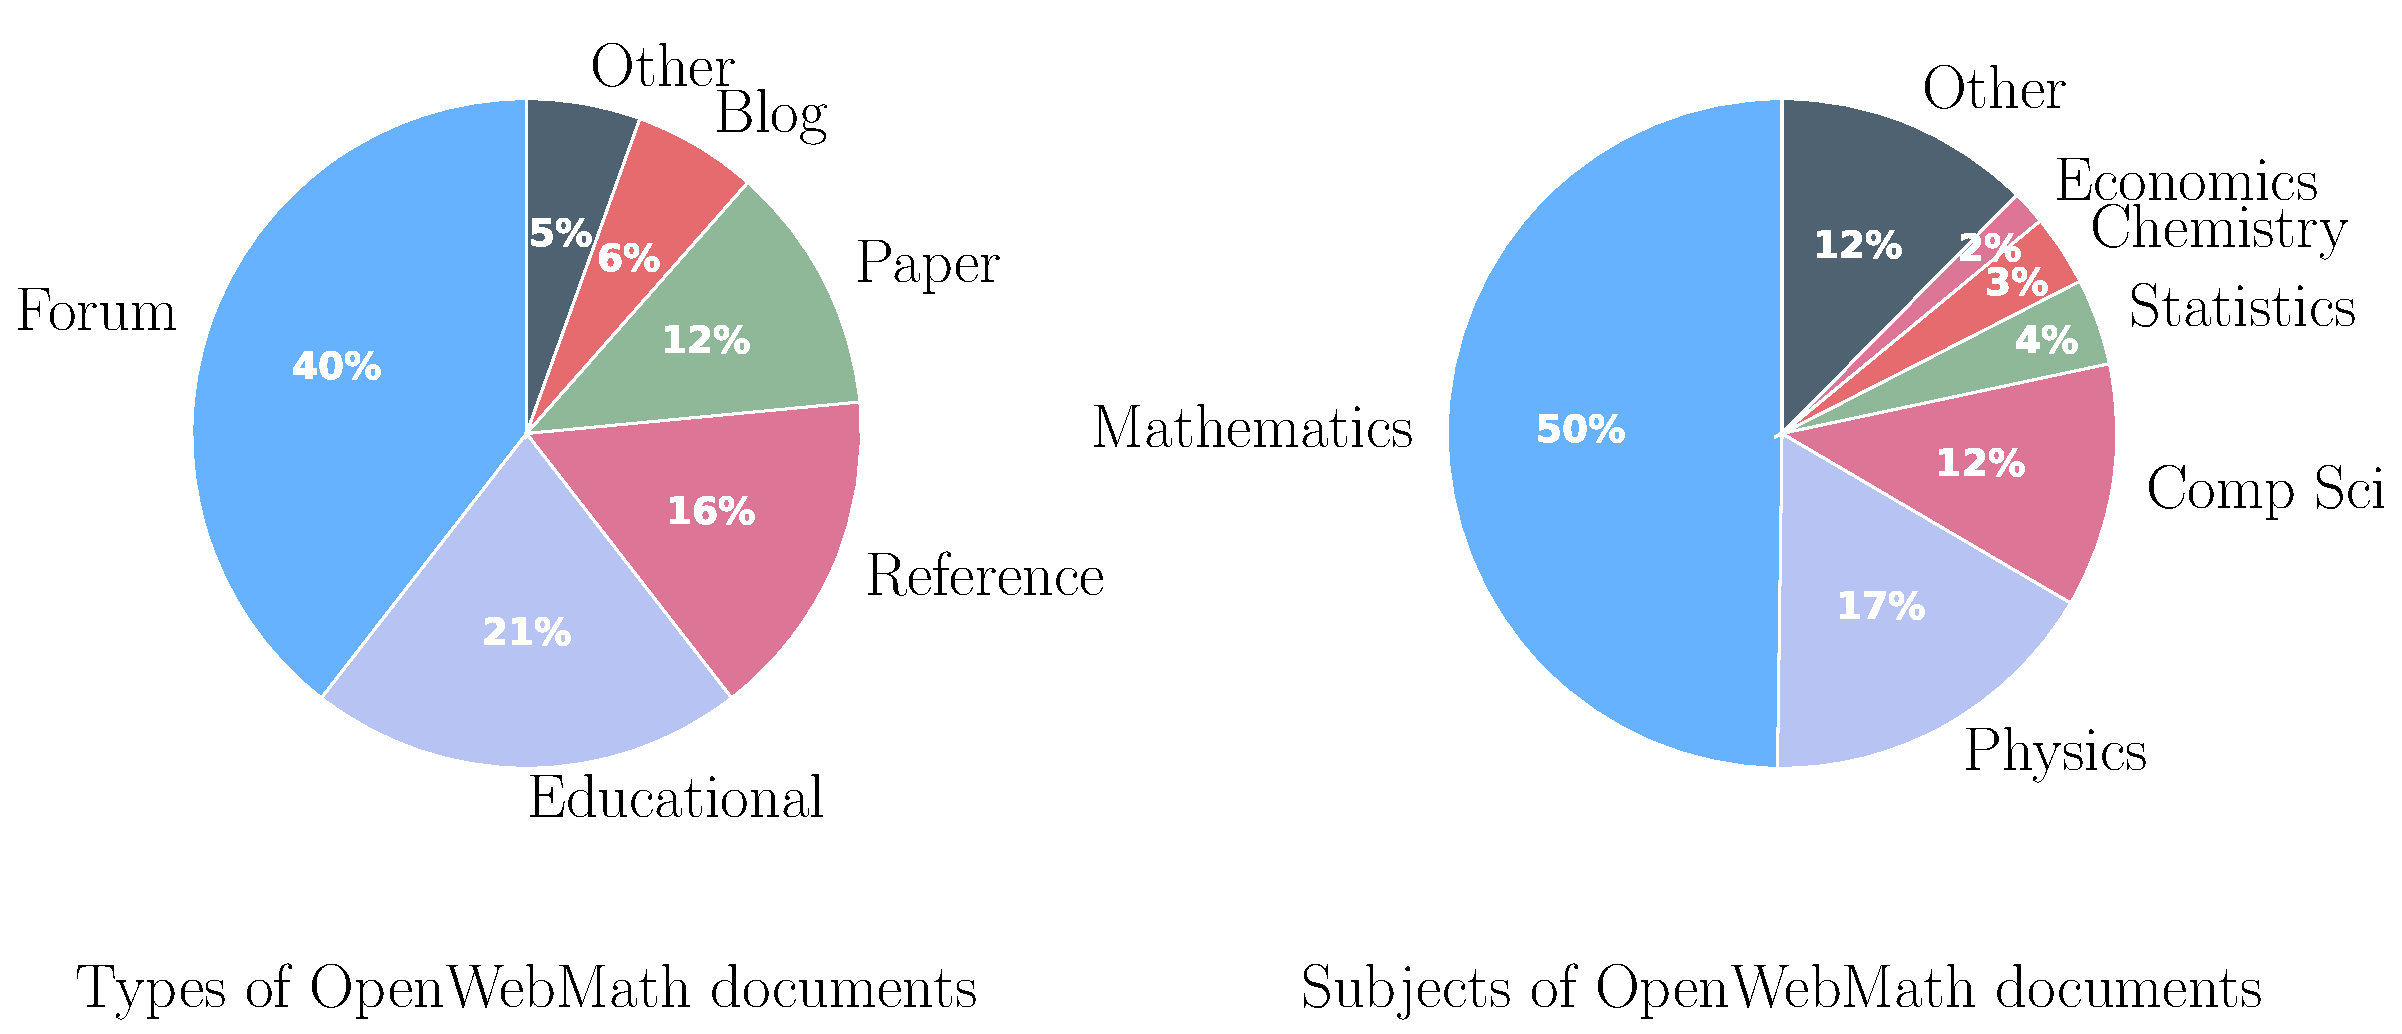
\includegraphics[width=\textwidth]{figures/pie_charts_combined.pdf}
    \end{center}
    \caption{\textbf{Left}: The documents in OpenWebMath are sourced from forum posts, educational content, reference pages, scientific papers, blogs, and more. Most content comes from Q\&A forums where users discuss how to solve problems. \textbf{Right}: The majority of the content in OpenWebMath is related to mathematics, but a large part is related to other technical subjects like Physics, Computer Science, Statistics, and more.}
    \label{fig:doublefig}
\end{figure}

\subsection{Web Data Processing Pipelines}
The pretraining of large language models requires large, diverse datasets. Data scraped from the web is one of the primary sources for such data. However, sources such as Common Crawl, which contains over 200 billion web pages, are known to have significant amounts of low-quality and duplicate content, requiring extensive filtering and deduplication to be suitable for training. Prior works such as C4 \citep{raffel2020exploring}, RefinedWeb \citep{refined-web}, CCNet \citep{wenzek2019ccnet}, The Pile \citep{gao2020pile}, and GPT-3 \citep{gpt3} introduce various pipelines for extracting quality data from Common Crawl for the purposes of language model training. These pipelines typically consist of three primary steps: text extraction, filtering, and deduplication.

\paragraph{Text extraction}
Extracting plain text from HTML files is a critical step in the creation of Common Crawl-based datasets. The easiest way to extract text from Common Crawl documents is to use the WET corresponding to each webpage, which contains pre-extracted plain text of the webpage. CCNet and C4 both use Common Crawl's WET files. However, the text extracted in WET files may contain too much boilerplate or miss out on important content such as \LaTeX{} equations. It is also possible to extract text directly from the raw HTML found in Common Crawl WARC files. The Pile uses an open source library called jusText \citep{justext} to extract text from HTML while RefinedWeb uses a library called Trafilatura \citep{barbaresi-2021-trafilatura}. These text extraction approaches differ in terms of extraction speed, customization, and their precision and recall for removing boilerplate content.

\paragraph{Filtering} 
The first layer of filtering often involves language identification \citep{wenzek2019ccnet}. Language filtering is used because certain other parts of the pipeline only work for specific languages, and is often done with simple linear classifiers such as from fastText \citep{joulin2016fasttext}. Quality filtering can be done with a combination of perplexity, classifier, and rule-based methods. CCNet uses a 5-gram Kneser-Ney language model implemented in the KenLM library \citep{heafield2011kenlm} trained on the target domain. The documents in the dataset are then sorted and filtered by their perplexity under this model. Other datasets such as the one used to train GPT-3 \citep{gpt3} use a classifier-based approach. This involves training a classifier on known-high-quality documents, such as those from Wikipedia, as positive examples and unfiltered documents from Common Crawl as negative examples. The classifier scores are used to filter low-quality documents from the dataset. Finally, rule-based approaches such as those used in C4 \citep{raffel2020exploring} and MassiveWeb \citep{gopher} involve removing pages with certain characters, too many or too few characters, too high a proportion of symbols, or those with an abnormal average word length. OpenMathWeb uses a mixture of these three approaches.

\paragraph{Deduplication} Given the periodic nature of Common Crawl snapshots and a general redundancy in web-sourced text, deduplication is an important processing step. Document-level near-deduplication (e.g., in \citep{gpt3, refined-web}) often employs MinHashLSH, an efficient algorithm for estimating the Jaccard similarity of documents. CCNet \citep{wenzek2019ccnet} uses paragraph-level deduplication, which can help to remove common boilerplate content found in WET text-extractions.